\documentclass{article}

\usepackage[a4paper, total={15cm, 25cm}]{geometry}
\usepackage[utf8]{inputenc}
\usepackage{amsmath}
\usepackage{amsfonts}
\usepackage{empheq}
\usepackage[most]{tcolorbox}
\newtcbox{\eqbox}[1][]{%
    nobeforeafter, math upper, tcbox raise base,
    enhanced, colframe=black, boxrule=1pt,
    #1}
\usepackage{float}
\usepackage{gensymb}

\def\*#1{\mathbf{#1}}

\title{Tecnologie Ottiche}
\author{Federico A. Corazza}
\date{}

\begin{document}
\maketitle

\section{Richiamo sulle equazioni di Maxwell}

\section{Equazioni di Fresnel}\label{section:eq_fresnel}
Siano $\*E_i$ e $\*E_r$ tangenti alla superficie (condizione \textbf{TE}), allora si ha che il campo elettrico nella zona 1 e 2 è pari a:
\begin{equation*}
\*E_1 = E_{0i} e^{i(\*k_i \*r-\omega_i t)} + E_{0r} e^{i(\*k_r \*r-\omega_r t)}
\end{equation*}
\begin{equation*}
\*E_2 = E_{0t} e^{i(\*k_t \*r-\omega_t t)}
\end{equation*}
Per le condizioni al contorno si ha che $\*E_{1t} = \*E_{2t}$ ovvero, per l'ipotesi fatta, $\*E_1 = \*E_2$. Da cui si ottiene:
\begin{equation*}
E_{0i} e^{i(\*k_i \*r-\omega_i t)} + E_{0r} e^{i(\*k_r \*r-\omega_r t)} = E_{0t} e^{i(\*k_t \*r-\omega_t t)}
\end{equation*}
Siccome questa relazione deve valere su qualsiasi punto del piano di separazione, gli esponenziali devono coincidere.
\begin{equation}\label{equation:exponentials}
\*k_i \*r-\omega_i t = \*k_r \*r-\omega_r t = \*k_t \*r-\omega_t t
\end{equation}
In particolare, la relazione deve valere anche per $\*r = \*0$.
\begin{equation}\label{equation:omega_is_constant_1}
-\omega_i t = -\omega_r t = -\omega_t t
\end{equation}
Dalla \eqref{equation:omega_is_constant_1} si ricava che le frequenze angolari devono essere uguali.
\begin{empheq}[box=\eqbox]{equation*}\label{equation:omega_is_constant_2}
\omega_i = \omega_r = \omega_t
\end{empheq}
Utilizzando nuovamente la \eqref{equation:exponentials} ponendo $t = 0$ si ha che:
\begin{equation}
\*k_i \*r = \*k_r \*r = \*k_t \*r
\end{equation}
Sottraendo membro a membro si ottiene:
\begin{equation}\label{equation:vet_donda_piano_dincidenza}
(\*k_i - \*k_r) \*r = (\*k_i - \*k_t) \*r = (\*k_r - \*k_t) \*r = 0
\end{equation}
Da cui si deduce che $\*k_i$, $\*k_r$ e $\*k_t$ appartengono al piano d'incidenza.\\
\\
Dalla \eqref{equation:vet_donda_piano_dincidenza} si deduce che:
\begin{equation}
k_i r \sin \theta_i = k_r r \sin \theta_r
\end{equation}
ovvero che
\begin{empheq}[box=\eqbox]{equation*}
\theta_i = \theta_r
\end{empheq}
Inoltre, utilizzando la seguente relazione:
\begin{equation}
k_i r \sin \theta_i = k_t r \sin \theta_t
\end{equation}
e utilizzando l'identità $k=\frac{\omega}{c}n$, si ottiene la legge di Snell.
\begin{empheq}[box=\eqbox]{equation*}
n_i \sin \theta_i = n_t \sin \theta_t
\end{empheq}
La legge di Snell descrive la relazione angolare tra onda incidente e onda trasmessa. Andiamo ora ad analizzare la relazione d'ampiezza e di fase.\\
\\
Come già visto, per onde \textbf{TE} si ha che la componente elettrica del campo è $E_{0i} + E_{0r} = E_{0t}$. Per la parte magnetica invece, se si utilizzano materiali completamente dielettrici, essa non viene influenzata; di conseguenza è possibile utilizzare la relazione tra E e B ($E = \frac{n}{c} B$) per ricavarne la relazione.\\
Riassumendo:
\begin{equation}
\begin{cases}
E_{0i} + E_{0r} = E_{0t}\\
n_1 E_{0i} \cos \theta_i + n_1 E_{0r} \cos \theta_i = n_2 E_{0t} \cos \theta_t
\end{cases}
\end{equation}
\\
Per onde TM
\begin{equation}
\begin{cases}
B_{0i} + B_{0r} = B_{0t} \Rightarrow n_1 E_{0i} + n_1 E_{0r} = n_2 E_{0t}\\
- E_{0i} \cos \theta_i + E_{0r} \cos \theta_i = - E_{0t} \cos \theta_t
\end{cases}
\end{equation}
\\
Poniamo $n=\frac{n_2}{n_1}$ con $n_1$ l'indice di rifrazione del mezzo da cui si parte e $n_2$ l'indice di rifrazione del mezza a cui si arriva e definiamo i coefficienti di riflessione.
\subsection{Coefficienti di Riflessione}
\begin{description}
\item [TE]
\begin{equation*}
r = \frac{E_{0r}}{E_{0i}} = \frac{\cos \theta_i - n \cos \theta_t}{\cos \theta_i + n \cos \theta_t}
\end{equation*}
applicando Pitagora e la legge di Snell
\begin{equation}
n \cos \theta_t = n\sqrt{1 - \sin^2 \theta_t} = \sqrt{n^2 - n^2 \sin^2 \theta_t} = \sqrt{n^2 - \sin^2 \theta_i}
\end{equation}
da cui si ottiene
\begin{empheq}[box=\eqbox]{equation}\label{equation:te_r}
r = \frac{\cos \theta_i - \sqrt{n^2 - \sin^2 \theta_i}}{\cos \theta_i + \sqrt{n^2 - \sin^2 \theta_i}}
\end{empheq}
\item [TM]
\begin{equation*}
r = \frac{E_{0r}}{E_0i} = \frac{n \cos \theta_i - \cos \theta_t}{n \cos \theta_i + \cos \theta_t}
\end{equation*}
seguendo gli stessi passaggi fatti per il caso TE si ottiene
\begin{empheq}[box=\eqbox]{equation}\label{equation:tm_r}
r = \frac{n^2 \cos \theta_i - \sqrt{n^2 - \sin^2 \theta_i}}{n^2 \cos \theta_i + \sqrt{n^2 - \sin^2 \theta_i}}
\end{empheq}
\end{description}

\subsection{Coefficienti di Trasmissione}
Analogamente definiamo i coefficienti di trasmissione t.
\begin{description}
\item [TE]
\begin{equation*}
t = \frac{E_{0t}}{E_{0i}}
\end{equation*}
\begin{empheq}[box=\eqbox]{equation}\label{equation:te_t}
t = \frac{2\cos \theta_i }{\cos \theta_i + \sqrt{n^2 - \sin^2 \theta_i}}
\end{empheq}
\item [TM]
\begin{equation*}
t = \frac{E_{0t}}{E_{0i}}
\end{equation*}
\begin{empheq}[box=\eqbox]{equation}\label{equation:tm_t}
t = \frac{2n \cos \theta_i }{n^2 \cos \theta_i + \sqrt{n^2 - \sin^2 \theta_i}}
\end{empheq}
\end{description}

\subsection{Relazione tra coefficienti di Riflessione e di Trasmissione}
Dalle relazioni \eqref{equation:te_r}, \eqref{equation:tm_r}, \eqref{equation:te_t} e \eqref{equation:tm_t} si ha che:
\begin{description}
\item [TE]
\begin{empheq}[box=\eqbox]{equation*}
t = r + 1
\end{empheq}
\item [TM]
\begin{empheq}[box=\eqbox]{equation*}
n t = r + 1
\end{empheq}
\end{description}

\subsection{Riflettività e Trasmittività}
Facciamo ora un bilancio energetico delle onde interessate, $P_i = P_r + P_t$, e definiamo la Riflettività R e la Trasmittività T.
\begin{equation*}
R = \frac{P_r}{P_i}
\end{equation*}
\begin{equation*}
T = \frac{P_t}{P_i}
\end{equation*}
da cui si può notare che $R + T = 1$.\\
Siccome la potenza incidente è data dall'intensità dell'onda su una certa superficie allora possiamo scrivere
\begin{equation*}
I_i A_i = I_r A_r + I_t A_t
\end{equation*}
tutte le aree in gioco avranno estensioni differenti tra di loro ma sul piano d'incidenza avranno la stessa proiezione, quindi
\begin{equation*}
I_i A \cos \theta_i = I_r A \cos \theta_r + I_t A \cos \theta_t
\end{equation*}
Semplificando l'area A e utilizzando la relazione generale di intensità di un'onda $I = \frac{\varepsilon_0}{2}cn E_0^2$ si ha
\begin{equation*}
n_1 E^2_{0i} \cos \theta_i = n_1 E^2_{0r} \cos \theta_i + n_2 E^2_{0t} \cos \theta_t
\end{equation*}
da cui si ottiene la seguente relazione che tornerà utile a breve
\begin{equation}\label{equation:R_T_E}
1 = \frac{E^2_{0r}}{E^2_{0i}} + n \frac{E^2_{0t}}{E^2_{0i}} \frac{\cos \theta_t}{\cos \theta_i} = r^2 + n t^2 \frac{\cos \theta_t}{\cos \theta_i}
\end{equation}
La Riflettività è dunque:
\begin{equation*}
R = \frac{P_r}{P_i} = \frac{I_r A_r}{I_i A_i} = \frac{E^2_{0r}}{E^2_{0i}}
\end{equation*}
quindi
\begin{empheq}[box=\eqbox]{equation}
R = r^2
\end{empheq}
Utilizzando ora la \eqref{equation:R_T_E} e il fatto che $R + T = 1$ la Trasmittività risulta essere
\begin{equation*}
T = 1 - R^2 = n t^2 \frac{\cos \theta_t}{\cos \theta_i}
\end{equation*}
quindi
\begin{empheq}[box=\eqbox]{equation}
T = n t^2 \frac{\cos \theta_t}{\cos \theta_i}
\end{empheq}

\subsection{Riflessione interna ed esterna}
Definiamo \textbf{riflessione esterna} quando l'onda incidente va dal mezzo a indice di rifrazione minore verso il mezzo con indice di rifrazione maggiore (\textbf{$n_1 < n_2$}) e quindi risulta \textbf{$n > 1$}.
Definiamo invece \textbf{riflessione interna} il caso opposto, ovvero quando l'onda incidente va dal mezzo a indice di rifrazione maggiore verso il mezzo con indice di rifrazione minore (\textbf{$n_1 > n_2$}) e quindi \textbf{$n < 1$}.

\begin{figure}[H]
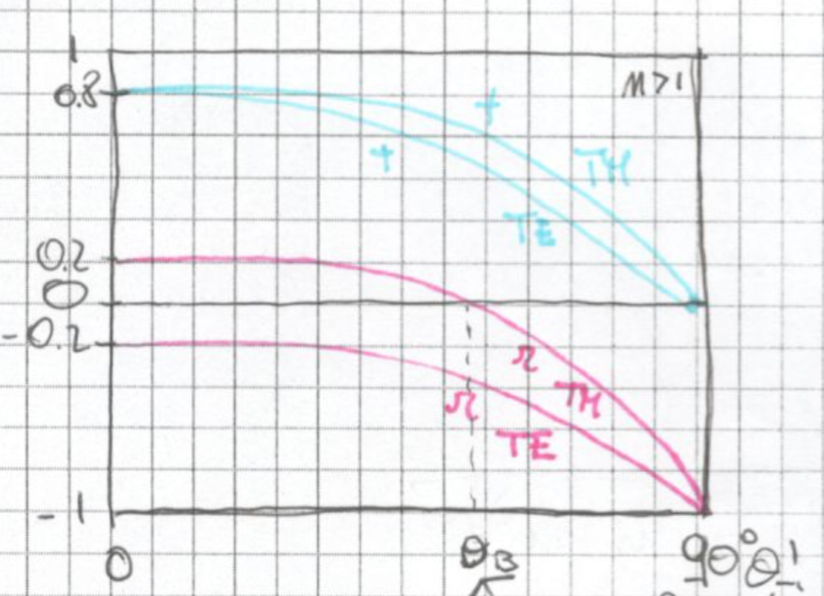
\includegraphics[width=8cm]{images/coeff_r_t_ext_rifl.png}
\centering
\end{figure}
\noindent
All'angolo di Brewster ($\theta_B$) non c'è riflessione.

\begin{figure}[H]
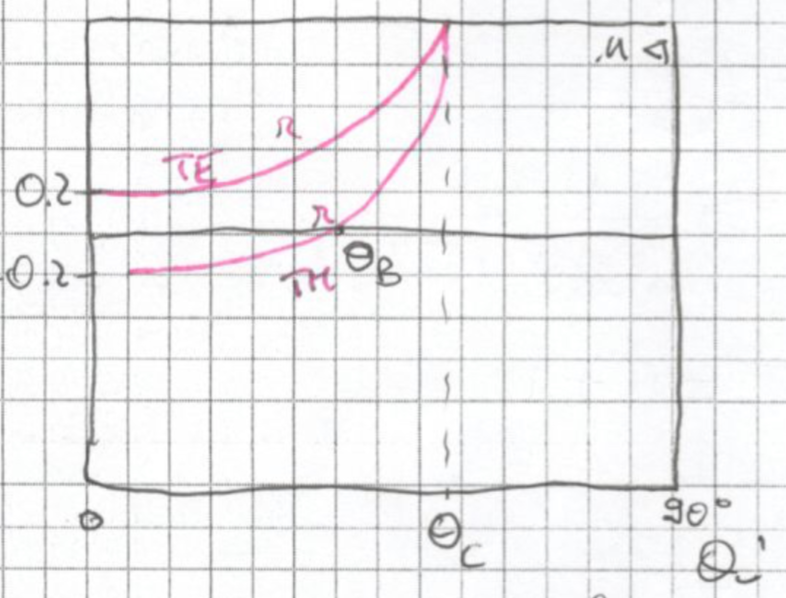
\includegraphics[width=8cm]{images/coeff_r_int_rifl.png}
\centering
\end{figure}
\noindent
Nel caso di riflessione interna oltre all'angolo critico ($\theta_C$) non c'è riflessione.
Si noti inoltre che per valori negativi l'onda riflessa subisce uno sfasamento di $\pi$.\\

\begin{figure}[H]
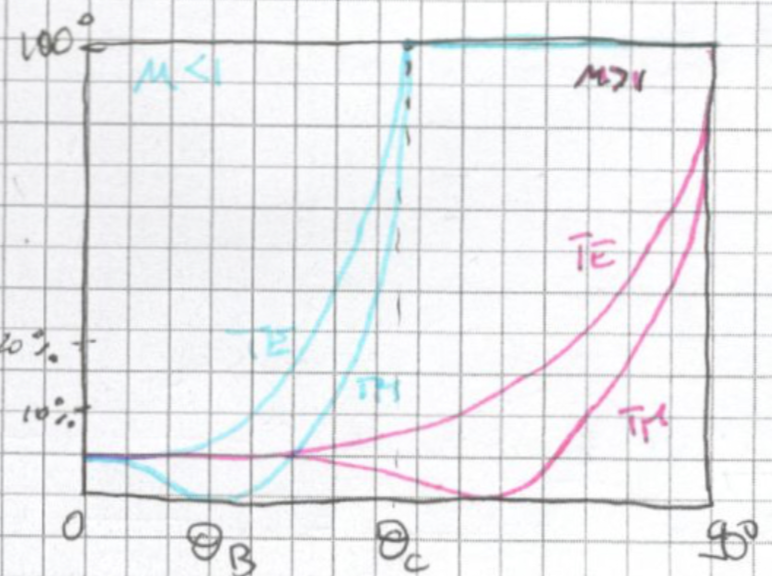
\includegraphics[width=8cm]{images/R_int_ext.png}
\centering
\end{figure}
\noindent
Se si prende $n_1 = 1$ (aria) e $n_2 = 1.5$ (vetro) allora la riflettività ad incidenza normale è
\begin{equation*}
R(\theta_i=0) = \left(\frac{1 - n}{1 + n}\right) \simeq 4\%
\end{equation*}

\subsection{Relazione di fase all'interfaccia}
\begin{description}
\item [TE] riflessione esterna
\begin{figure}[H]
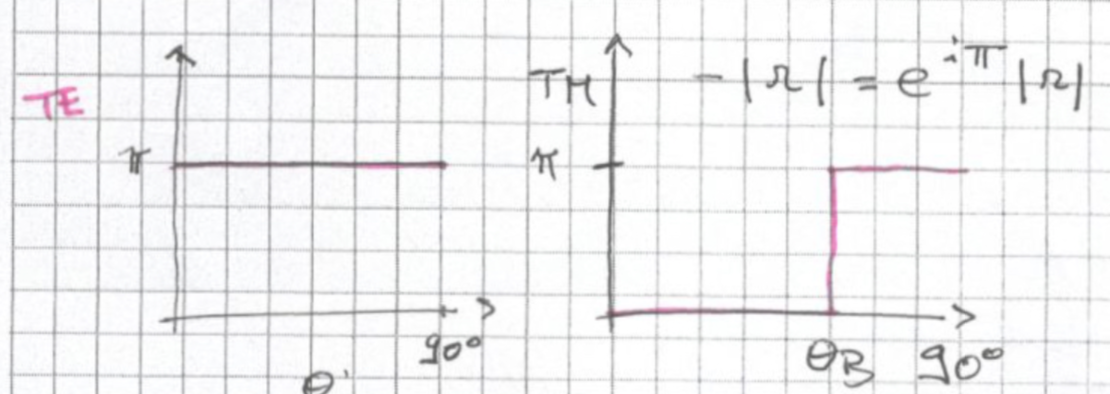
\includegraphics[width=8cm]{images/ext_rifl_fase.png}
\centering
\end{figure}
\item [TM] riflessione interna
\begin{figure}[H]
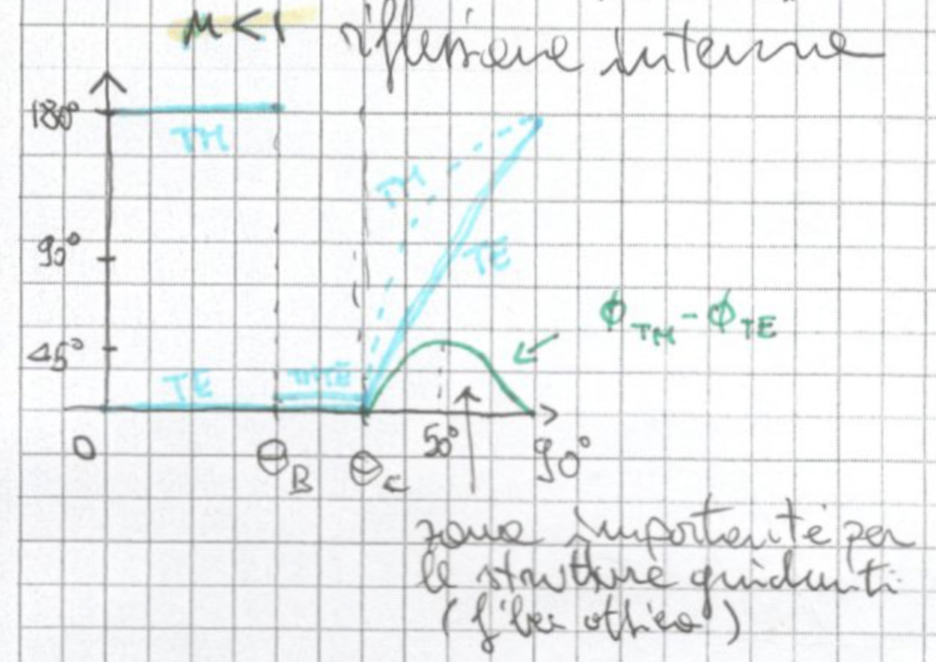
\includegraphics[width=8cm]{images/int_rifl_fase.png}
\centering
\end{figure}
\noindent
A circa $50\degree$ la differenza di fase è circa $45\degree$.
\end{description}

\subsection{Rombo di Fresnel}
Considerando un'onda e.m. \textit{polarizzata linearmente} a $45\degree$ nel verso uscente dalla figura. Possiamo considerare le componenti come separate: una parte in trasversa elettrica l'altra in trasversa magnetica. Esse subiscono una doppia riflessione a $50\degree$ che ne cambia la fase di $45\degree$. Quindi tra di loro le onde hanno una differenza di fase di $90\degree$ che, una volta ricombinate in un'unica onda, risulta in una \textit{polarizzazione circolare}.
\begin{figure}[H]
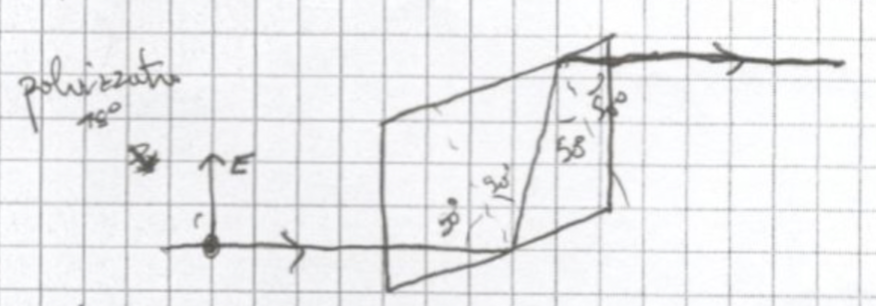
\includegraphics[width=8cm]{images/rombo_fresnel.png}
\centering
\end{figure}

\newpage

\section{Teoria dei multistrati}
Attraverso l'utilizzo di molti strati di dielettrici è possibile realizzare specchi, sfruttando quanto trovato nel paragrafo \ref{section:eq_fresnel}.\\
Analizziamo ad esempio un sistema composto da un substrato di indice di rifrazione $n_s$ con un rivestimento (film) con indice di rifrazione $n_f$.\\
Invece di inseguire ogni onda riflessa e trasmessa nel sistema, analizziamo la situazione lungo l'asse $x$ nel suo insieme.
\begin{equation}
\begin{cases}
E_a = E_0 + E_{r1} = E_{t1} + E_{i1}\\
E_b = E_{i2} + E_{r2} = E_{t2}
\end{cases}
\end{equation}
\begin{equation*}
\begin{cases}
B_a = B_0 \cos \theta_0 - B_{r1} \cos \theta_0 = B_{t1} \cos \theta_{t1} + B_{i1} \cos \theta_{t1} \\
B_b = B_{i2} \cos \theta_{t1} - B_{r2} \cos \theta_{t1} = B_{t2} \cos \theta_{t2}
\end{cases}
\end{equation*}
definiamo $\gamma_0 = \frac{n_0}{c} \cos \theta_0$, $\gamma_1 = \frac{n_1}{c} \cos \theta_{t1}$ e $\gamma_s = \frac{n_s}{c} \cos \theta_{t2}$.
\begin{equation}
\begin{cases}
B_a = \gamma_0 (E_0 - E_{r1}) = \gamma_1 (E_{t1} - E_{i1})\\
B_b = \gamma_1 (E_{i2} - E_{r2}) = \gamma_s E_{t2}
\end{cases}
\end{equation}
All'interno dello stesso mezzo l'ampiezza rimane invariata ma può presentarsi uno sfasamento di fase $\delta$.
\begin{equation}
\delta = k_0 \Delta = (\frac{2\pi}{\lambda_0}) n_1 d \cos \theta_{t1}
\end{equation}
Da cui abbiamo che:
\begin{equation}
E_{i2} = E_{t1} e^{i \delta} \qquad  E_{r2} = E_{i1} e^{-i \delta}
\end{equation}
Sostituiamo nella equazioni \eqref{} e \eqref{} ottenendo
\begin{equation}
E_{t1} = \frac{\gamma_1 E_b + B_b}{2 \gamma_1}e^{-i\delta} \qquad E_{i1} = \frac{\gamma_1 E_b - B_b}{2 \gamma_1}e^{+i\delta}
\end{equation}
Utilizzando le identità $\cos \delta = \frac{e^{i\delta} + e^{-i\delta}}{2}$ e $\sin \delta = \frac{e^{i\delta} - e^{-i\delta}}{2i}$ si ha:
\begin{equation}
\begin{cases}
E_a = E_b \cos \delta + B_b(-i\frac{\sin \delta}{\gamma_1}) \\
B_a = E_b(-i \gamma_1 \sin \delta) + B_b \cos \delta
\end{cases}
\end{equation}
In forma vettoriale:
\[
\left| \begin{array}{c}
E_a \\
B_a 
\end{array} \right| = 
\left| \begin{array}{cc}
\cos \delta & i\frac{\sin \delta}{\gamma_1} \\
i \gamma_1 \sin \delta & \cos \delta
\end{array} \right|
\left| \begin{array}{c}
E_b \\
B_b 
\end{array} \right|
\]
utilizzando la seguente forma generale
\[
\left| \begin{array}{c}
E_a \\
B_a 
\end{array} \right| = 
\left| \begin{array}{cc}
m_{11} & m_{12} \\
m_{21} & m_{22}
\end{array} \right|
\left| \begin{array}{c}
E_b \\
B_b 
\end{array} \right|
\]
notiamo che ogni strato è relazionato con quello adiacente. Di conseguenza è possibile mettere in relazione il primo strato con l'ultimo attraverso il prodotto tra matrici.
\[
\left| \begin{array}{c}
E_a \\
B_a 
\end{array} \right| = 
M_1 M_2 ... M_{N-1} M_N
\left| \begin{array}{c}
E_b \\
B_b 
\end{array} \right|
\]
Questa relazione è molto utile perché quello che ci interessa fare è calcolare la riflessione e la trasmissione dell'intera struttura.\\
Calcoliamo quindi i coefficienti di riflessione e trasmissione per il caso precedente (substrato + film).
\begin{empheq}[box=\eqbox]{equation}
r = \frac{\gamma_0 m_{11} + \gamma_0 \gamma_sm_{12} - m_{21} - \gamma_s m_{22}}{\gamma_0 m_{11} + \gamma_0 \gamma_s m_{12} + m_{21} + \gamma_s m_{22}}
\end{empheq}
\begin{empheq}[box=\eqbox]{equation}
t = \frac{2 \gamma_0}{\gamma_0 m_{11} + \gamma_0 \gamma_s m_{12} + m_{21} + \gamma_s m_{22}}
\end{empheq}
L'unica differenza tra i coefficienti tra onde TE e TM è il valore di $\gamma_1$ infatti:
\begin{description}
\item [TE]
\begin{equation}
\gamma_1 = \frac{n}{c} \cdot \cos \theta_{t1}
\end{equation}
\item [TM]
\begin{equation}
\gamma_1 = \frac{n}{c} \cdot \frac{1}{\cos \theta_{t1}}
\end{equation}
\end{description}
Calcoliamo ora la riflettività per un'onda ad incidenza normale. 
\begin{equation}
R = |r|^2 = \frac{A^2 + B^2}{C^2 + D^2} = \frac{n_1^2(n_0 - n_s)^2 \cos^2 \delta + (n_0 n_s - n_1^2)^2 \sin^2 \delta}{n_1^2(n_0 + n_s)^2 \cos^2 \delta + (n_0 n_s + n_1^2)^2 \sin^2 \delta}
\end{equation}
\begin{equation}
\delta = \frac{2\pi}{\lambda_0} \Delta = \frac{2\pi}{\lambda_0} n_1 d
\end{equation}
con $\Delta$ indicato il cammino ottico.\\
I massimi e i minimi della riflettività si trovano per $\Delta = (2N +1)\frac{\lambda_0}{4}$. Generalmente per ragioni costruttive si prende lo strato più sottile possibile per minimizzare i costi di produzione.
\begin{equation*}
d_{max/min} = \frac{\lambda_0}{4n_1} = \frac{\lambda}{4}
\end{equation*}
Uno strato antiriflesso con questo spessore è detto a \textit{lambda quarti}.\\
\begin{equation*}
\delta = \frac{\pi}{2}
\end{equation*}
I massimi e i minimi della riflettività sono dunque dati da:
\begin{equation}
R_{max/min} = \left( \frac{n_0 n_s - n_1^2}{n_0 n_s + n_1^2} \right)^2
\end{equation}
La riflettività è nulla per $n_1 = \sqrt{n_0 n_s}$. Siccome non si ha grande libertà di scelta tra i materiali con indici di rifrazione diversa non è facile creare strati completamente riflettenti. Inoltre, con questa metodologia la riflessione è minimizzata solamente per un intorno di una lunghezza d'onda in particolare. Vediamo successivamente come, aggiungendo un ulteriore strato, sia possibile diminuire ulteriormente la riflettività.

\subsection{Sistema antiriflesso a due strati}
Consideriamo due strati antiriflesso a \textit{lambda quarti} con le rispettivi spessori: $d_1 = \frac{\lambda_0}{4n_1}$ e $d_2 = \frac{\lambda_0}{4n_2}$.
Descriviamo i due strati attraverso le seguenti matrici e ne calcoliamo l'equivalente attraverso il prodotto di queste.
\[
M_1 = \left| \begin{array}{cc}
0 & -\frac{i}{\gamma_1} \\
-\frac{i}{\gamma_1} & 0
\end{array} \right|
\qquad
M_2 = \left| \begin{array}{cc}
0 & -\frac{i}{\gamma_2} \\
-\frac{i}{\gamma_2} & 0
\end{array} \right|
\qquad
M_{tot} = M_1 M_2 = \left| \begin{array}{cc}
-\frac{\gamma_2}{\gamma_1} & 0 \\
0 & -\frac{\gamma_1}{\gamma_2}
\end{array} \right|
\]
Dalla matrice equivalente è possibile ricavare il coefficiente di riflessione e quindi la riflettività.
\begin{equation}
R = \left( \frac{n_0 n_2^2 - n_s n_1^2}{n_0 n_2^2 + n_s n_1^2} \right)^2
\end{equation}
Per avere riflettività nulla si deve avere $n_0 n_2^2 - n_s n_1^ = 0$ ovvero $\frac{n_2}{n_1} = \sqrt{\frac{n_s}{n_0}}$. Se $n_0 = 1$ allora si ha $\frac{n_2}{n_1} = \sqrt{n_s} > 1 \rightarrow n_2 > n_1$. Con l'aggiunta di uno strato siamo riusciti ad abbassare ulteriormente la riflettività ma come detto precedentemente sarebbe ancora più utile avere una \textit{banda} antiriflesso invece che per una singola $\lambda$.

\subsection{Sistema antiriflesso a tre strati}
Consideriamo ora tre strati antiriflesso a \textit{lambda quarti} di spessore: $d_i = \frac{\lambda_0}{4n_i}$ con indici di rifrazione basso, alto, basso rispettivamente e scriviamo la matrice equivalente del sistema ottico:
\[
M_{tot} = M_1 M_2 M_3 = \left| \begin{array}{cc}
0 & i\frac{\gamma_2}{\gamma_1 \gamma_3} \\
i\frac{\gamma_1 \gamma_3}{\gamma_2} & 0
\end{array} \right|
\]
Sostituendo nella formula del coefficiente di riflessione si ottiene che la riflettività è nulla per $\frac{n_1 n_3}{n_2} = \sqrt{n_0 n_s}$.
In questo modo si ha una banda su cui la riflettività è trascurabile.

\subsection{Specchi multi-dielettrici}
Vediamo invece ora come attraverso diversi strati di materiali con indici di rifrazione diversi sia possibile creare sistemi ottici riflettenti, ovvero degli specchi dielettrici.\\
In particolare consideriamo una serie di N coppie di strati ognuna composta da uno strato ad indice di rifrazione alta e uno ad indice di rifrazione bassa che indicheremo con $n_H$ e $n_L$ rispettivamente.\\
Ogni coppia può essere descritta attraverso la seguente matrice:
\begin{equation*}
M_{HL} = M_H M_L = \left| \begin{array}{cc}
0 & -\frac{i}{\gamma_H} \\
-i\gamma_H & 0
\end{array} \right|
\left| \begin{array}{cc}
0 & -\frac{i}{\gamma_L} \\
-i\gamma_L & 0
\end{array} \right|
= \left| \begin{array}{cc}
-\frac{\gamma_L}{\gamma_H} & 0\\
0 & -\frac{\gamma_H}{\gamma_L}
\end{array} \right|
\end{equation*}
Nel suo complesso, il sistema ottico può essere descritto da:
\begin{equation}
M_{tot} = \left| \begin{array}{cc}
-\frac{\gamma_L}{\gamma_H} & 0\\
0 & -\frac{\gamma_H}{\gamma_L}
\end{array} \right|^N
\end{equation}
Ricaviamo il coefficiente di riflessione:
\begin{equation*}
r = \frac{n_0(-\frac{n_L}{n_H})^N - n_s(-\frac{n_H}{n_L})^N}{n_0(-\frac{n_L}{n_H})^N + n_s(-\frac{n_H}{n_L})^N}
\end{equation*}
e la riflettività:
\begin{equation*}
R = \left[\frac{(\frac{n_0}{n_s})(\frac{n_L}{n_H})^{2N} - 1}{(\frac{n_0}{n_s})(\frac{n_L}{n_H})^{2N} + 1}\right]^2
\end{equation*}

\section{Interferometri}
\subsection{Relazioni di Stokes}
Riprendiamo il caso di un'onda incidente all'interfaccia tra due materiali con indice di rifrazione $n_1$ e $n_2$ rispettivamente. L'ampiezza dell'onda incidente che indicheremo con $E_i$ verrà separata in un'onda riflessa e in un'onda trasmessa di ampiezze $rE_i$ e $tE_i$ ciascuna con r e t i coefficienti di riflessione e trasmissione.
\begin{equation*}
r = \frac{E_r}{E_i} \qquad t = \frac{E_t}{E_i}
\end{equation*}
Applichiamo il principio di reversibilità dei raggi e consideriamo due onde incidenti, una corrispondente all'onda riflessa nel caso precedente e l'altra corrispondente all'onda trasmessa nel caso precedente. Per l'onda incidente dal mezzo 1 al mezzo 2 si avrà anche in questo caso una separazione in due onde. Quella riflessa avrà ampiezza $r'rE_i$, quella trasmessa $t'rE_i$. Analogamente per l'onda incidente dal mezzo 2 al mezzo 1 si ha un'onda riflessa di ampiezza $r^2E_i$ e una trasmessa di ampiezza $trE_i$.\\
Mettendo in relazione i due casi si ottiene:
\begin{equation*}
\begin{cases}
E_i = t'tE_i + r^2E_i = (t't + r^2)E_i \\
0 = r'tE_i + rtE_i = (r' + r)tE_i
\end{cases}
\end{equation*}
Da cui si ricavano le \textbf{Relazioni di Stokes}:
\begin{equation}
\begin{cases}
t' t + r^2 = 1\\
r' = -r
\end{cases}
\end{equation}

\subsection{Interferometro di Fabry-Perot}
Consideriamo ora due superfici parallele sulle quali viene fatta incidere un'onda ad un certo angolo $\theta_0$. Su entrambe le superfici si avranno riflessioni e trasmissioni multiple come mostrato in figura.
\begin{figure}[H]
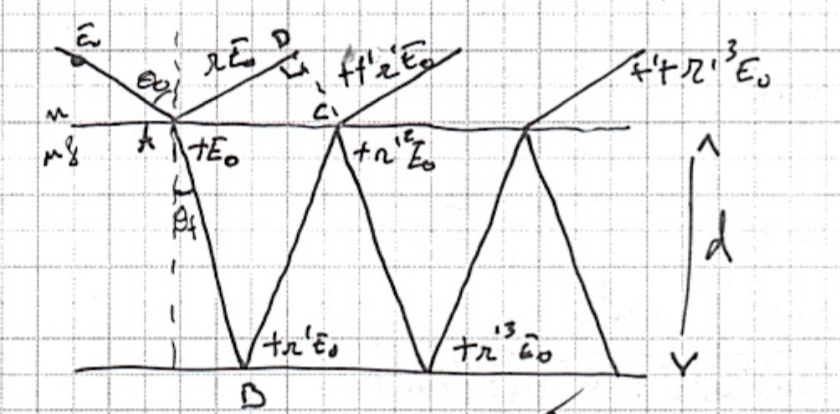
\includegraphics[width=8cm]{images/interf_facce_piane.png}
\centering
\end{figure}
\noindent
Cerchiamo di trovare $E_{r,tot}$. Tutti i raggi riflessi alla prima interfaccia presentano una differenza di fase dovuta dal diverso cammino ottico.
\begin{equation*}
\Delta = \frac{2d}{\cos \theta_t} n_f [1 - \sin^2 \theta_t]
\end{equation*}
\begin{empheq}[box=\eqbox]{equation}
\Delta = 2d n_f \cos \theta_t
\end{empheq}
Da cui si ricava la differenza di fase $\delta = k\Delta$:
\begin{empheq}[box=\eqbox]{equation}
\overline{\delta} = \frac{4\pi}{\lambda_0} d n_f \cos \theta_t
\end{empheq}
Con la convenzione $\overline{\delta} = 2 \delta = 2 \cdot \frac{2\pi}{\lambda_0} d n_f \cos \theta_t$.
Se l'onda incidente è $E_0$ allora le onde riflesse saranno:
\begin{equation*}
\begin{split}
& E_1 = rE_0 e^{i\overline{\delta}} \\
& E_2 = tt'r'E_0 e^{i\overline{\delta}}\\
& E_3 = tt'r'^3 E_0 e^{i2\overline{\delta}}\\
& E_4 = tt'r'^5 E_0 e^{i3\overline{\delta}}\\
& \qquad ...
\end{split}
\end{equation*}
Guardando le equazioni precedenti attentamente si può notare come esse possano essere riassunte nella forma
\begin{equation*}
E_N = tt'r'^{(2N-3)} E_0 e^{i(N-1)\overline{\delta}} \qquad \forall N > 1
\end{equation*}
Questa espressione non vale per il termine $N = 1$ in quanto l'onda in questione non attraversa mai l'interfaccia.\\
Quindi possiamo riassumere il discorso calcolando l'onda riflessa complessiva.
\begin{equation*}
E_{r,tot} = rE_0 + \sum_{N=2}^\infty tt'r'^{2N-3} E_0 e^{i(N-1)\overline{\delta}}
\end{equation*}
Raccogliamo $E_0$ ed estraiamo un $r' e^{i\overline{\delta}}$ dalla sommatoria.
\begin{equation*}
E_{r,tot} = E_0 \left[r + (tt'r'e^{i\overline{\delta}}) \sum_{N=2}^\infty r'^{2N-4} E_0 e^{i(N-2)\overline{\delta}} \right]
\end{equation*}
Ora possiamo effettuare la sostituzione $x = r'^2 e^{i\overline{\delta}}$ enotare che la si tratta di una serie geometrica $\sum_{N=2}^\infty x^{N-2}$ la quale per $|x| < 1$ converge a $\frac{1}{1-x}$.\\
Riscriviamo sostituendo la sommatoria e sfruttando le relazioni di Stokes:
\begin{equation*}
E_{r,tot} = E_0 \left[r - \frac{(1-r^2)r e^{i\overline{\delta}}}{1 - r^2 e^{i\delta}} \right]
\end{equation*}
Sostituendo le superfici parallele considerate con 2 lamine di vetro si costruisce un interferometro di Fabry-Perot per cui valgono le considerazioni fatte fino ad ora.\\
Calcoliamo ora la riflettività.
\begin{equation*}
R_{tot} = \left| \frac{E_{r,tot}}{E_0} \right|^2 = \frac{2R(1 - \cos \overline{\delta})}{1 + R^2 -2R \cos \overline{\delta}}
\end{equation*}
con R riflettività della superficie.\\
Dalla riflettività si può calcolare la trasmittività $T_{tot} = 1 - R_{tot}$
\begin{equation}
T_{tot} = \frac{1}{1 + \frac{4R \sin^2 \frac{\overline{\delta}}{2}}{1-R^2}}
\end{equation}
Definiamo coefficiente di \textit{finesse}
\begin{empheq}[box=\eqbox]{equation}
F = \frac{4R}{(1-R)^2}
\end{empheq}
Da cui si trova la trasmittività dell'interferometro di Fabry-Perot
\begin{empheq}[box=\eqbox]{equation}
T_{tot} = \frac{1}{1 + F \sin^2 \frac{\overline{\delta}}{2}}
\end{empheq}
La quale è massima quando $\sin^2 \frac{\overline{\delta}}{2} = 0$ ovvero quando $\overline{\delta} = 2m\pi$ e minima quando $\overline{\delta} = (2m+1)\pi$ e $F \rightarrow +\infty$.\\
Definiamo \textit{free spectral range} la distanza tra un picco d'interferenza di ordine $m$ e di ordine $m+1$. In particolare:
\begin{equation*}
\Delta \nu_{fsr} = \nu_{m+1} - \nu_m = \frac{(m+1)c}{2n_fd} - \frac{mc}{2n_fd} = \frac{c}{2n_fd}
\end{equation*}
\begin{empheq}[box=\eqbox]{equation}
\Delta \nu_{fsr} = \frac{c}{2n_fd}
\end{empheq}
Definiamo inoltre lo spessore a mezza altezza di un picco $\Delta \overline{\delta}_c$. Ovvero quando $t=\frac{1}{2}$ il ché accade per $\sin^2 \frac{\overline{\delta}_c}{2} = \frac{1}{\sqrt{F}}$. Siccome F è molto grande possiamo approssimare e dire che $\Delta \overline{\delta}_c = \frac{4}{\sqrt{F}}$. In termini della frequenza:
\begin{empheq}[box=\eqbox]{equation}
\Delta \nu_c = \frac{c}{\pi \sqrt{F}n_fd}
\end{empheq}
Definiamo infine la \textit{finesse} (diversa dal coefficiente di Finesse)
\begin{empheq}[box=\eqbox]{equation}
\mathcal{F} = \frac{\Delta \nu_{fsr}}{\Delta \nu_c} = \frac{\pi}{2} \sqrt{F}
\end{empheq}
Un buon interferometro ha $\Delta \nu_{fsr}$ larghe e $\Delta \nu_c$ strette (alti valori di $F$). La finesse è limitata dalla rugosità delle superfici utilizzate.Infatti un'indeterminazione nello spessore della superficie genera un'indeterminazione nello sfasamento.
\begin{equation*}
\Delta d = \frac{\lambda}{M}
\end{equation*}
Questa relazione indica la qualità di una superficie definita in funzione della lunghezza d'onda. Più M è grande migliore è la superficie.
\begin{equation*}
\Delta \overline{\delta}_{\text{non planare}} = \frac{4\pi}{\lambda} \Delta d = \frac{4\pi}{M}
\end{equation*}
\begin{equation*}
\Delta \overline{\delta}_c = \frac{4}{\sqrt{F}}
\end{equation*}
\begin{equation*}
\Delta \overline{\delta}_\text{non planare} > \Delta \overline{\delta}_c
\end{equation*}
\begin{equation}
\mathcal{F} = \frac{\Delta \nu_{fsr}}{\Delta \nu_c} = \frac{\Delta \overline{\delta}_{fsr}}{\Delta \overline{\delta}_\text{non planare}} = \frac{2\pi}{\frac{4\pi}{M}} = \frac{M}{2}
\end{equation}
Se $M=100$, il massimo valore di finesse possibile è $\mathcal{F} = 50$.

\subsubsection{Interferometro di Fabry-Perot come analizzatore di spettro}
Consideriamo un sistema ottico composto da due supporti ottici piani paralleli con uno strato antiriflesso sui lati interni e la possibilità di modificare la distanza tra questi.\\
Muovendo gli specchi.
\begin{empheq}[box=\eqbox]{equation}
R = \frac{\lambda}{\Delta \lambda_{min}}
\end{empheq}

\subsection*{Interferometro di Michelson}
\subsection*{Variazioni dell'interferometro di Michelson}
\subsubsection*{Interferometro di Twyman-Green}
\subsubsection*{Interferometro di Mach-Zender}


\end{document}
